% !TEX root = main.tex

本课程采用书目Alfred V. Aho, Monica S. Lam, Ravi Sethi, Jeffrey D. Ullman, \emph{Compilers: Principles, Techniques \& Tools (2nd ed)},即大名鼎鼎的龙书。

\section{简介}
编译器的几个阶段如下,前端包括词法(lexical)、语法(syntax)、语义(semantic)分析,中端IR生成、优化,后端代码生成。
\begin{figure}[H]
\centering
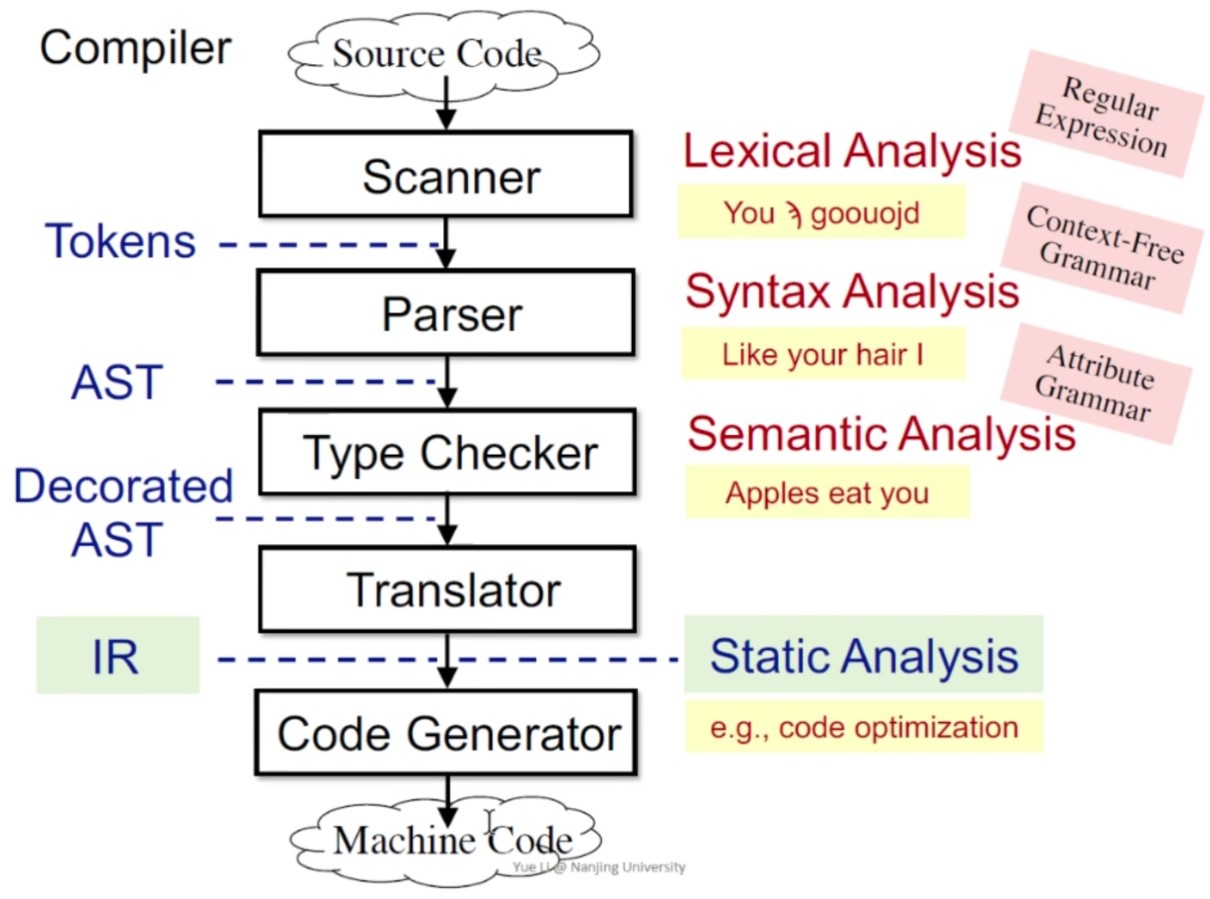
\includegraphics[width=0.6\linewidth]{fig/compiler_flow.jpg}
\end{figure}